% Supplementary Material for the Cognition and Emotion submission (published via Figshare).
% Tables are generated by analysis/05_report_numbers.py; figures by analysis/03, 04 and 06 (confirmatory sample).
% Build from this directory: latexmk -pdf supplement.tex
\documentclass[11pt,a4paper]{article}
\usepackage[british]{babel}
\usepackage[T1]{fontenc}
\usepackage{newtxtext,newtxmath} % Times-style; heavier strokes than Latin Modern, easier to read on screens
\usepackage[margin=2.2cm]{geometry}
\usepackage{booktabs,array,threeparttable,graphicx,amsmath,csquotes,float}
\usepackage[hidelinks]{hyperref}
\usepackage[font=small,labelfont=bf]{caption}
\graphicspath{{../results/confirmatory/figures/}{figures/}}
\renewcommand{\thetable}{S\arabic{table}}
\renewcommand{\thefigure}{S\arabic{figure}}
% Written by analysis/05_report_numbers.py - do not edit by hand.
\newcommand{\val}[1]{\ifcsname val:#1\endcsname\csname val:#1\endcsname\else\errmessage{Unknown value #1}\fi}
\expandafter\def\csname val:n_completed\endcsname{130}
\expandafter\def\csname val:n_excluded\endcsname{6}
\expandafter\def\csname val:n_primary\endcsname{124}
\expandafter\def\csname val:n_excl_disrupted\endcsname{3}
\expandafter\def\csname val:n_excl_freetext\endcsname{2}
\expandafter\def\csname val:n_excl_erratic\endcsname{1}
\expandafter\def\csname val:n_cohort_two\endcsname{19}
\expandafter\def\csname val:n_cohort_three\endcsname{20}
\expandafter\def\csname val:n_cohort_four\endcsname{85}
\expandafter\def\csname val:n_age\endcsname{121}
\expandafter\def\csname val:age_mean\endcsname{34.2}
\expandafter\def\csname val:age_sd\endcsname{12.0}
\expandafter\def\csname val:age_min\endcsname{18}
\expandafter\def\csname val:age_max\endcsname{76}
\expandafter\def\csname val:n_female\endcsname{59}
\expandafter\def\csname val:n_male\endcsname{62}
\expandafter\def\csname val:n_sex_missing\endcsname{3}
\expandafter\def\csname val:n_mouse\endcsname{80}
\expandafter\def\csname val:n_trackpad\endcsname{43}
\expandafter\def\csname val:n_stricter\endcsname{96}
\expandafter\def\csname val:n_sparse\endcsname{24}
\expandafter\def\csname val:n_one_check\endcsname{5}
\expandafter\def\csname val:n_not_attentive\endcsname{3}
\expandafter\def\csname val:n_without_rejected\endcsname{120}
\expandafter\def\csname val:n_rejection_set\endcsname{4}
\expandafter\def\csname val:n_exploratory_completed\endcsname{23}
\expandafter\def\csname val:n_exploratory\endcsname{21}
\expandafter\def\csname val:height_fear_mean\endcsname{3.77}
\expandafter\def\csname val:height_fear_sd\endcsname{1.73}
\expandafter\def\csname val:height_fear_median\endcsname{4}
\expandafter\def\csname val:sticsa_pre_mean\endcsname{13.76}
\expandafter\def\csname val:sticsa_pre_sd\endcsname{3.56}
\expandafter\def\csname val:sticsa_pre_median\endcsname{13}
\expandafter\def\csname val:sticsa_post_mean\endcsname{20.55}
\expandafter\def\csname val:sticsa_post_sd\endcsname{7.29}
\expandafter\def\csname val:sticsa_post_median\endcsname{18}
\expandafter\def\csname val:sticsa_change_mean\endcsname{6.79}
\expandafter\def\csname val:sticsa_change_sd\endcsname{6.60}
\expandafter\def\csname val:sticsa_change_median\endcsname{5}
\expandafter\def\csname val:anxiety_overall_mean\endcsname{5.18}
\expandafter\def\csname val:anxiety_overall_sd\endcsname{1.33}
\expandafter\def\csname val:anxiety_overall_median\endcsname{5}
\expandafter\def\csname val:concern_safety_mean\endcsname{6.13}
\expandafter\def\csname val:concern_safety_sd\endcsname{1.30}
\expandafter\def\csname val:concern_safety_median\endcsname{7}
\expandafter\def\csname val:body_intensity_mean\endcsname{4.64}
\expandafter\def\csname val:body_intensity_sd\endcsname{1.60}
\expandafter\def\csname val:body_intensity_median\endcsname{5}
\expandafter\def\csname val:arousal_baseline_mean\endcsname{43.13}
\expandafter\def\csname val:arousal_baseline_sd\endcsname{15.80}
\expandafter\def\csname val:arousal_baseline_median\endcsname{43.8}
\expandafter\def\csname val:arousal_rise_mean\endcsname{67.14}
\expandafter\def\csname val:arousal_rise_sd\endcsname{14.79}
\expandafter\def\csname val:arousal_rise_median\endcsname{68.9}
\expandafter\def\csname val:arousal_plateau_mean\endcsname{80.91}
\expandafter\def\csname val:arousal_plateau_sd\endcsname{15.01}
\expandafter\def\csname val:arousal_plateau_median\endcsname{83.1}
\expandafter\def\csname val:arousal_return_mean\endcsname{53.89}
\expandafter\def\csname val:arousal_return_sd\endcsname{19.42}
\expandafter\def\csname val:arousal_return_median\endcsname{54.8}
\expandafter\def\csname val:arousal_whole_film_mean\endcsname{61.23}
\expandafter\def\csname val:arousal_whole_film_sd\endcsname{10.99}
\expandafter\def\csname val:arousal_whole_film_median\endcsname{60.6}
\expandafter\def\csname val:valence_baseline_mean\endcsname{50.58}
\expandafter\def\csname val:valence_baseline_sd\endcsname{14.55}
\expandafter\def\csname val:valence_baseline_median\endcsname{52.0}
\expandafter\def\csname val:valence_rise_mean\endcsname{39.58}
\expandafter\def\csname val:valence_rise_sd\endcsname{19.06}
\expandafter\def\csname val:valence_rise_median\endcsname{38.5}
\expandafter\def\csname val:valence_plateau_mean\endcsname{29.13}
\expandafter\def\csname val:valence_plateau_sd\endcsname{23.10}
\expandafter\def\csname val:valence_plateau_median\endcsname{23.9}
\expandafter\def\csname val:valence_return_mean\endcsname{50.84}
\expandafter\def\csname val:valence_return_sd\endcsname{20.44}
\expandafter\def\csname val:valence_return_median\endcsname{51.7}
\expandafter\def\csname val:valence_whole_film_mean\endcsname{41.89}
\expandafter\def\csname val:valence_whole_film_sd\endcsname{14.67}
\expandafter\def\csname val:valence_whole_film_median\endcsname{41.9}
\expandafter\def\csname val:H1:report\endcsname{$t$(123) = 11.46, $p$ < .001, $d_z$ = 1.03, 95\% CI [0.81, 1.25]}
\expandafter\def\csname val:H1:effect\endcsname{$d_z$ = 1.03 [0.81, 1.25]}
\expandafter\def\csname val:H1:est\endcsname{1.03}
\expandafter\def\csname val:H1:diff\endcsname{6.79}
\expandafter\def\csname val:H1:diffabs\endcsname{6.79}
\expandafter\def\csname val:H2a:report\endcsname{$t$(123) = 14.67, $p_\mathrm{Holm}$ < .001, $d_z$ = 1.32, 95\% CI [1.07, 1.56]}
\expandafter\def\csname val:H2a:effect\endcsname{$d_z$ = 1.32 [1.07, 1.56]}
\expandafter\def\csname val:H2a:est\endcsname{1.32}
\expandafter\def\csname val:H2a:diff\endcsname{24.01}
\expandafter\def\csname val:H2a:diffabs\endcsname{24.01}
\expandafter\def\csname val:H2b:report\endcsname{$t$(123) = 19.77, $p_\mathrm{Holm}$ < .001, $d_z$ = 1.78, 95\% CI [1.49, 2.06]}
\expandafter\def\csname val:H2b:effect\endcsname{$d_z$ = 1.78 [1.49, 2.06]}
\expandafter\def\csname val:H2b:est\endcsname{1.78}
\expandafter\def\csname val:H2b:diff\endcsname{37.78}
\expandafter\def\csname val:H2b:diffabs\endcsname{37.78}
\expandafter\def\csname val:H2c:report\endcsname{$t$(123) = $-$14.70, $p_\mathrm{Holm}$ < .001, $d_z$ = $-$1.32, 95\% CI [$-$1.56, $-$1.08]}
\expandafter\def\csname val:H2c:effect\endcsname{$d_z$ = $-$1.32 [$-$1.56, $-$1.08]}
\expandafter\def\csname val:H2c:est\endcsname{$-$1.32}
\expandafter\def\csname val:H2c:diff\endcsname{$-$27.02}
\expandafter\def\csname val:H2c:diffabs\endcsname{27.02}
\expandafter\def\csname val:H2d:report\endcsname{$t$(123) = $-$9.85, $p_\mathrm{Holm}$ < .001, $d_z$ = $-$0.88, 95\% CI [$-$1.09, $-$0.68]}
\expandafter\def\csname val:H2d:effect\endcsname{$d_z$ = $-$0.88 [$-$1.09, $-$0.68]}
\expandafter\def\csname val:H2d:est\endcsname{$-$0.88}
\expandafter\def\csname val:H2d:diff\endcsname{$-$21.44}
\expandafter\def\csname val:H2d:diffabs\endcsname{21.44}
\expandafter\def\csname val:H3arousal:report\endcsname{$r$ = .993, 95\% CI [.990, .996]}
\expandafter\def\csname val:H3arousal:effect\endcsname{$r$ = .993 [.990, .996]}
\expandafter\def\csname val:H3arousal:est\endcsname{.99}
\expandafter\def\csname val:H3valence:report\endcsname{$r$ = .937, 95\% CI [.893, .966]}
\expandafter\def\csname val:H3valence:effect\endcsname{$r$ = .937 [.893, .966]}
\expandafter\def\csname val:H3valence:est\endcsname{.94}
\expandafter\def\csname val:H4a:report\endcsname{$\rho$ = .08, 95\% CI [$-$.09, .26], $p$ = .355, $p_\mathrm{Holm}$ = .355}
\expandafter\def\csname val:H4a:effect\endcsname{$\rho$ = .08 [$-$.09, .26]}
\expandafter\def\csname val:H4a:est\endcsname{.08}
\expandafter\def\csname val:H4b:report\endcsname{$\rho$ = $-$.32, 95\% CI [$-$.46, $-$.16], $p$ < .001, $p_\mathrm{Holm}$ = .001}
\expandafter\def\csname val:H4b:effect\endcsname{$\rho$ = $-$.32 [$-$.46, $-$.16]}
\expandafter\def\csname val:H4b:est\endcsname{$-$.32}
\expandafter\def\csname val:H4c:report\endcsname{$\rho$ = .18, 95\% CI [.00, .35], $p$ = .049, $p_\mathrm{Holm}$ = .098}
\expandafter\def\csname val:H4c:effect\endcsname{$\rho$ = .18 [.00, .35]}
\expandafter\def\csname val:H4c:est\endcsname{.18}
\expandafter\def\csname val:H5a:report\endcsname{$\rho$ = .24, 95\% CI [.05, .41], $p$ = .008, $p_\mathrm{Holm}$ = .008}
\expandafter\def\csname val:H5a:effect\endcsname{$\rho$ = .24 [.05, .41]}
\expandafter\def\csname val:H5a:est\endcsname{.24}
\expandafter\def\csname val:H5b:report\endcsname{$\rho$ = $-$.38, 95\% CI [$-$.51, $-$.23], $p$ < .001, $p_\mathrm{Holm}$ < .001}
\expandafter\def\csname val:H5b:effect\endcsname{$\rho$ = $-$.38 [$-$.51, $-$.23]}
\expandafter\def\csname val:H5b:est\endcsname{$-$.38}
\expandafter\def\csname val:H6a:report\endcsname{$\rho$ = .56, 95\% CI [.44, .67], $p$ < .001, $p_\mathrm{Holm}$ < .001}
\expandafter\def\csname val:H6a:effect\endcsname{$\rho$ = .56 [.44, .67]}
\expandafter\def\csname val:H6a:est\endcsname{.56}
\expandafter\def\csname val:H6b:report\endcsname{$\rho$ = .34, 95\% CI [.15, .50], $p$ < .001, $p_\mathrm{Holm}$ < .001}
\expandafter\def\csname val:H6b:effect\endcsname{$\rho$ = .34 [.15, .50]}
\expandafter\def\csname val:H6b:est\endcsname{.34}
\expandafter\def\csname val:H2:absrange\endcsname{0.88--1.78}
\expandafter\def\csname val:H1:wilcoxon\endcsname{$T$ = 197, $p$ < .001}
\expandafter\def\csname val:n_floor_pre\endcsname{45}
\expandafter\def\csname val:pct_floor_pre\endcsname{36}
\expandafter\def\csname val:n_increase\endcsname{109}
\expandafter\def\csname val:n_nochange\endcsname{7}
\expandafter\def\csname val:n_decrease\endcsname{8}
\expandafter\def\csname val:n_fear_top\endcsname{20}
\expandafter\def\csname val:n_fear_seven\endcsname{2}
\expandafter\def\csname val:rel:arousal\endcsname{.992}
\expandafter\def\csname val:rel:valence\endcsname{.979}
\expandafter\def\csname val:edge1:est\endcsname{262}
\expandafter\def\csname val:edge1:reg\endcsname{262}
\expandafter\def\csname val:edge1:ci\endcsname{[133, 271]}
\expandafter\def\csname val:edge2:est\endcsname{467}
\expandafter\def\csname val:edge2:reg\endcsname{470}
\expandafter\def\csname val:edge2:ci\endcsname{[317, 475]}
\expandafter\def\csname val:edge3:est\endcsname{660}
\expandafter\def\csname val:edge3:reg\endcsname{692}
\expandafter\def\csname val:edge3:ci\endcsname{[631, 690]}
\expandafter\def\csname val:confirmatory_commit\endcsname{63d042d}
\expandafter\def\csname val:seed\endcsname{20261004}
\expandafter\def\csname val:python_version\endcsname{3.13.7}
\expandafter\def\csname val:version:numpy\endcsname{2.5.3}
\expandafter\def\csname val:version:pandas\endcsname{3.0.6}
\expandafter\def\csname val:version:scipy\endcsname{1.18.1}
\expandafter\def\csname val:version:matplotlib\endcsname{3.11.2}
\expandafter\def\csname val:version:statsmodels\endcsname{0.15.0}
\expandafter\def\csname val:n_demo\endcsname{121}
\expandafter\def\csname val:n_demo_female\endcsname{59}
\expandafter\def\csname val:n_demo_male\endcsname{62}
\expandafter\def\csname val:change_female_mean\endcsname{7.17}
\expandafter\def\csname val:change_male_mean\endcsname{6.44}
\expandafter\def\csname val:agesex:change_sex\endcsname{0.66 [$-$1.77, 3.08], $p$ = .593}
\expandafter\def\csname val:agesex:change_age\endcsname{0.24 [$-$0.78, 1.25], $p$ = .645}
\expandafter\def\csname val:agesex:arousal:sex_x_segment\endcsname{$\chi^2$(3) = 0.28, $p$ = .964}
\expandafter\def\csname val:agesex:arousal:sex_x_segment:check\endcsname{$F$(3, 120) = 0.08, $p$ = .969}
\expandafter\def\csname val:agesex:arousal:age_x_segment\endcsname{$\chi^2$(3) = 4.92, $p$ = .178}
\expandafter\def\csname val:agesex:arousal:age_x_segment:check\endcsname{$F$(3, 120) = 2.13, $p$ = .100}
\expandafter\def\csname val:agesex:arousal:female_minus_male\endcsname{$-$0.50 [$-$4.47, 3.47], $p$ = .806}
\expandafter\def\csname val:agesex:arousal:per_10_years\endcsname{$-$1.26 [$-$2.88, 0.37], $p$ = .129}
\expandafter\def\csname val:agesex:valence:sex_x_segment\endcsname{$\chi^2$(3) = 0.72, $p$ = .869}
\expandafter\def\csname val:agesex:valence:sex_x_segment:check\endcsname{$F$(3, 120) = 0.43, $p$ = .734}
\expandafter\def\csname val:agesex:valence:age_x_segment\endcsname{$\chi^2$(3) = 1.84, $p$ = .607}
\expandafter\def\csname val:agesex:valence:age_x_segment:check\endcsname{$F$(3, 120) = 0.50, $p$ = .682}
\expandafter\def\csname val:agesex:valence:female_minus_male\endcsname{$-$4.46 [$-$9.91, 0.99], $p$ = .108}
\expandafter\def\csname val:agesex:valence:per_10_years\endcsname{$-$0.74 [$-$2.96, 1.47], $p$ = .511}
\expandafter\def\csname val:agesex:valence_rise_diff\endcsname{$-$6.43 points [$-$13.19, 0.34], $p$ = .062}
\expandafter\def\csname val:items:dz_min\endcsname{0.52}
\expandafter\def\csname val:items:dz_max\endcsname{1.17}
\expandafter\def\csname val:items:pholm_max\endcsname{< .001}
\expandafter\def\csname val:items:rank1:label\endcsname{heart beats fast}
\expandafter\def\csname val:items:rank1:dz\endcsname{1.17}
\expandafter\def\csname val:items:rank2:label\endcsname{trembly, shaky}
\expandafter\def\csname val:items:rank2:dz\endcsname{0.80}
\expandafter\def\csname val:items:rank3:label\endcsname{breathing fast, shallow}
\expandafter\def\csname val:items:rank3:dz\endcsname{0.77}
\expandafter\def\csname val:items:rank4:label\endcsname{muscles tense}
\expandafter\def\csname val:items:rank4:dz\endcsname{0.72}
\expandafter\def\csname val:items:rank5:label\endcsname{dizzy}
\expandafter\def\csname val:items:rank5:dz\endcsname{0.71}
\expandafter\def\csname val:items:rank6:label\endcsname{face hot}
\expandafter\def\csname val:items:rank6:dz\endcsname{0.66}
\expandafter\def\csname val:items:rank7:label\endcsname{butterflies in stomach}
\expandafter\def\csname val:items:rank7:dz\endcsname{0.64}
\expandafter\def\csname val:items:rank8:label\endcsname{palms clammy}
\expandafter\def\csname val:items:rank8:dz\endcsname{0.60}
\expandafter\def\csname val:items:rank9:label\endcsname{throat dry}
\expandafter\def\csname val:items:rank9:dz\endcsname{0.54}
\expandafter\def\csname val:items:rank10:label\endcsname{muscles weak}
\expandafter\def\csname val:items:rank10:dz\endcsname{0.52}
\expandafter\def\csname val:items:rank11:label\endcsname{arms and legs stiff}
\expandafter\def\csname val:items:rank11:dz\endcsname{0.52}
\expandafter\def\csname val:task:valence\endcsname{20}
\expandafter\def\csname val:task:arousal\endcsname{88}


\title{Supplementary Material\\[4pt]\large Moment-to-Moment Affect During Film-Induced Somatic Anxiety}
\date{}
\author{}

\begin{document}
\maketitle

\section*{S0. The Rating Task}

\begin{figure}[H]
\centering

\includegraphics[width=0.75\textwidth]{task_illustration.png}
\caption{The rating screen during the film (illustration). Participants moved the dot within the affect grid in the
lower right corner with the mouse: left to right for unpleasant to pleasant, down to up for low to high activation
(arousal). The image is a composite of the film frame at 10:36, during the scene in which a member of the group is held
by one hand over the edge, with the rating grid redrawn as it appears in the task; the dot marks the confirmatory
sample's mean rating at that moment (valence \val{task:valence}, arousal \val{task:arousal}). Film frame from
Tikhomirov (2017).}
\label{fig:task}
\end{figure}

\section*{S1. Sample and Descriptive Statistics}

Table~\ref{tab:sample} describes the exploratory sample, all confirmatory completers and the primary confirmatory
sample; Table~\ref{tab:descriptives} gives descriptive statistics for all measures used in the confirmatory tests.

\begin{table}[tbp]
\caption{Sample Characteristics}
\label{tab:sample}
\begin{threeparttable}
\small\linespread{1}\selectfont
\begin{tabular}{@{}l*{3}{>{\centering\arraybackslash}p{2.6cm}}@{}}
\toprule
Characteristic & Exploratory, usable & Confirmatory, all completers & Confirmatory, primary sample \\
\midrule
$n$ & 21 & 130 & 124 \\
Age, years, $M$ ($SD$) & 35.0 (12.6) & 34.1 (11.9) & 34.2 (12.0) \\
\hspace{1em}Range & 19--60 & 18--76 & 18--76 \\
Sex, $n$ (\%) & & & \\
\hspace{1em}Female & 13 (62) & 62 (48) & 59 (48) \\
\hspace{1em}Male & 8 (38) & 64 (49) & 62 (50) \\
\hspace{1em}Not available\tnote{a} & 0 (0) & 4 (3) & 3 (2) \\
Input device, $n$ (\%) & & & \\
\hspace{1em}Mouse & 15 (71) & 86 (66) & 80 (65) \\
\hspace{1em}Trackpad & 6 (29) & 43 (33) & 43 (35) \\
\hspace{1em}Other & 0 (0) & 1 (1) & 1 (1) \\
Everyday fear of heights (1--7), $M$ ($SD$) & 3.52 (1.72) & 3.72 (1.73) & 3.77 (1.73) \\
STICSA somatic, pre-film (11--44), $M$ ($SD$) & 12.24 (1.81) & 13.72 (3.51) & 13.76 (3.56) \\
Failed one attention check, $n$ (\%) & 0 (0) & 5 (4) & 5 (4) \\
Excluded under registered rules, $n$ & 0 & 6 & 0 \\
\bottomrule
\end{tabular}
\vspace{4pt}
\begin{tablenotes}[para,flushleft]
{\small\textit{Note.} Exploratory sample: pilot and cohort 1, usable under the registered rules (reference curve for H3). Confirmatory sample: cohorts 2--4. Age and sex are Prolific profile data; input device is self-reported. STICSA = State-Trait Inventory for Cognitive and Somatic Anxiety, state somatic subscale. \tnote{a}Prolific withholds demographic data for rejected submissions.}
\end{tablenotes}
\end{threeparttable}
\end{table}

\begin{table}[tbp]
\caption{Descriptive Statistics, Primary Confirmatory Sample}
\label{tab:descriptives}
\begin{threeparttable}
\linespread{1}\selectfont
\begin{tabular}{@{}lccccc@{}}
\toprule
Measure & Scale & $M$ & $SD$ & $Mdn$ & Range \\
\midrule
\multicolumn{6}{l}{\textit{Before the film}} \\
\hspace{1em}Everyday fear of heights & 1--7 & 3.77 & 1.73 & 4.00 & 1--7 \\
\hspace{1em}STICSA somatic, pre-film & 11--44 & 13.76 & 3.56 & 13.00 & 11--27 \\
\multicolumn{6}{l}{\textit{After the film}} \\
\hspace{1em}STICSA somatic, post-film & 11--44 & 20.55 & 7.29 & 18.00 & 11--44 \\
\hspace{1em}STICSA somatic change (post $-$ pre) &  & 6.79 & 6.60 & 5.00 & $-$6--32 \\
\hspace{1em}Overall anxiety while watching & 1--7 & 5.18 & 1.33 & 5.00 & 1--7 \\
\hspace{1em}Concern for the climbers' safety & 1--7 & 6.13 & 1.30 & 7.00 & 1--7 \\
\hspace{1em}Intensity of bodily sensations & 1--7 & 4.64 & 1.60 & 5.00 & 1--7 \\
\multicolumn{6}{l}{\textit{Continuous arousal}} \\
\hspace{1em}Baseline (0:00--4:22) & 0--100 & 43.13 & 15.80 & 43.76 & 5.9--76.4 \\
\hspace{1em}Rise (4:22--7:50) & 0--100 & 67.14 & 14.79 & 68.91 & 22.5--96.1 \\
\hspace{1em}Plateau (7:50--11:32) & 0--100 & 80.91 & 15.01 & 83.07 & 24.2--100.0 \\
\hspace{1em}Return (11:32--13:28) & 0--100 & 53.89 & 19.42 & 54.76 & 13.3--96.9 \\
\hspace{1em}Whole film & 0--100 & 61.23 & 10.99 & 60.58 & 21.2--86.7 \\
\multicolumn{6}{l}{\textit{Continuous valence}} \\
\hspace{1em}Baseline (0:00--4:22) & 0--100 & 50.58 & 14.55 & 51.96 & 12.6--85.2 \\
\hspace{1em}Rise (4:22--7:50) & 0--100 & 39.58 & 19.06 & 38.52 & 0.2--83.3 \\
\hspace{1em}Plateau (7:50--11:32) & 0--100 & 29.13 & 23.10 & 23.89 & 0.0--100.0 \\
\hspace{1em}Return (11:32--13:28) & 0--100 & 50.84 & 20.44 & 51.67 & 0.6--97.9 \\
\hspace{1em}Whole film & 0--100 & 41.89 & 14.67 & 41.91 & 4.6--86.5 \\
\bottomrule
\end{tabular}
\vspace{4pt}
\begin{tablenotes}[para,flushleft]
{\small\textit{Note.} $N$ = 124. Range is the observed minimum--maximum. Continuous ratings are participant means of the 1-Hz series within each registered segment (film time in min:s); valence 0 = unpleasant, 50 = neutral, 100 = pleasant; arousal 0 = low, 100 = high. STICSA = State-Trait Inventory for Cognitive and Somatic Anxiety, state somatic subscale.}
\end{tablenotes}
\end{threeparttable}
\end{table}


\section*{S2. Confirmatory Tests and Sensitivity Analyses}

Table~\ref{tab:confirmatory} lists all preregistered tests in the primary sample, and Table~\ref{tab:sensitivity}
repeats them in the two preregistered sensitivity samples. The stricter-engagement sample
($n$~=~\val{n_stricter}) additionally excluded sparse raters (fewer than one rating bout per minute, or more than 180~s
without input; \val{n_sparse}), participants who failed one attention check (\val{n_one_check}) and participants who
reported not watching attentively (\val{n_not_attentive}); these groups overlap. The second sample
($n$~=~\val{n_without_rejected}) excluded the \val{n_rejection_set} participants whose Prolific submissions were
rejected for behaviour on the free-text page but who passed the registered exclusion rules. Figure~\ref{fig:segments}
shows segment means and Figure~\ref{fig:correlations} the individual-difference tests.

\begin{table}[tbp]
\caption{Preregistered Confirmatory Tests, Primary Sample}
\label{tab:confirmatory}
\begin{threeparttable}
\footnotesize\linespread{1}\selectfont\setlength{\tabcolsep}{3.5pt}
\begin{tabular}{@{}l>{\raggedright\arraybackslash}p{3.0cm}cllll@{}}
\toprule
Hypothesis & Prediction & Test statistic & Effect size [95\% CI] & $p$ & $p_\mathrm{Holm}$ & Supported \\
\midrule
H1 & STICSA somatic: post $>$ pre & $t$(123) = 11.46 & $d_z$ = 1.03 [0.81, 1.25] & $<$ .001 & -- & Yes \\
\addlinespace
H2a & Arousal: rise $>$ baseline & $t$(123) = 14.67 & $d_z$ = 1.32 [1.07, 1.56] & $<$ .001 & $<$ .001 & Yes \\
H2b & Arousal: plateau $>$ baseline & $t$(123) = 19.77 & $d_z$ = 1.78 [1.49, 2.06] & $<$ .001 & $<$ .001 & Yes \\
H2c & Arousal: return $<$ plateau & $t$(123) = $-$14.70 & $d_z$ = $-$1.32 [$-$1.56, $-$1.08] & $<$ .001 & $<$ .001 & Yes \\
H2d & Valence: plateau $<$ baseline & $t$(123) = $-$9.85 & $d_z$ = $-$0.88 [$-$1.09, $-$0.68] & $<$ .001 & $<$ .001 & Yes \\
\addlinespace
H3 arousal & Arousal curve replicates & -- & $r$ = .993 [.990, .996] & -- & -- & Yes \\
H3 valence & Valence curve replicates & -- & $r$ = .937 [.893, .966] & -- & -- & Yes \\
\addlinespace
H4a & Fear of heights, plateau arousal (+) & -- & $\rho$ = .08 [$-$.09, .26] & .355 & .355 & No \\
H4b & Fear of heights, plateau valence ($-$) & -- & $\rho$ = $-$.32 [$-$.46, $-$.16] & $<$ .001 & .001 & Yes \\
H4c & Fear of heights, STICSA change (+) & -- & $\rho$ = .18 [.00, .35] & .049 & .098 & No \\
\addlinespace
H5a & STICSA change, whole-film arousal (+) & -- & $\rho$ = .24 [.05, .41] & .008 & .008 & Yes \\
H5b & STICSA change, whole-film valence ($-$) & -- & $\rho$ = $-$.38 [$-$.51, $-$.23] & $<$ .001 & $<$ .001 & Yes \\
\addlinespace
H6a & Overall anxiety, STICSA change (+) & -- & $\rho$ = .56 [.44, .67] & $<$ .001 & $<$ .001 & Yes \\
H6b & Overall anxiety, plateau arousal (+) & -- & $\rho$ = .34 [.15, .50] & $<$ .001 & $<$ .001 & Yes \\
\bottomrule
\end{tabular}
\vspace{4pt}
\begin{tablenotes}[para,flushleft]
{\small\textit{Note.} $N$ = 124. H1 and H2: paired $t$ tests with $d_z$ and exact 95\% CIs (noncentral $t$). H3: Pearson $r$ between the confirmatory and exploratory group-mean series (808 one-second values), 95\% CI from a circular block bootstrap (30-s blocks, 5,000 resamples); supported if the lower bound exceeds .50. H4--H6: Spearman $\rho$ with percentile bootstrap 95\% CIs (5,000 resamples). Holm correction within H2 (four tests), H4 (three), H5 (two) and H6 (two); H1 is a single test. All tests two-sided; a directional hypothesis counts as supported only if significant in the predicted direction.}
\end{tablenotes}
\end{threeparttable}
\end{table}

\begin{table}[tbp]
\caption{Preregistered Tests Repeated in the Sensitivity Samples}
\label{tab:sensitivity}
\begin{threeparttable}
\footnotesize\linespread{1}\selectfont\setlength{\tabcolsep}{3.5pt}
\begin{tabular}{@{}llccc@{}}
\toprule
Hypothesis & Effect & Primary ($n$ = 124) & Stricter engagement ($n$ = 96) & Rejection set removed ($n$ = 120) \\
\midrule
H1 & $d_z$ & 1.03 ($p$ < .001) & 1.09 ($p$ < .001) & 1.02 ($p$ < .001) \\
H2a & $d_z$ & 1.32 ($p_\mathrm{Holm}$ < .001) & 1.51 ($p_\mathrm{Holm}$ < .001) & 1.43 ($p_\mathrm{Holm}$ < .001) \\
H2b & $d_z$ & 1.78 ($p_\mathrm{Holm}$ < .001) & 1.94 ($p_\mathrm{Holm}$ < .001) & 1.85 ($p_\mathrm{Holm}$ < .001) \\
H2c & $d_z$ & $-$1.32 ($p_\mathrm{Holm}$ < .001) & $-$1.65 ($p_\mathrm{Holm}$ < .001) & $-$1.39 ($p_\mathrm{Holm}$ < .001) \\
H2d & $d_z$ & $-$0.88 ($p_\mathrm{Holm}$ < .001) & $-$0.88 ($p_\mathrm{Holm}$ < .001) & $-$0.87 ($p_\mathrm{Holm}$ < .001) \\
H3 arousal & $r$ & .993 (lower .990) & .990 (lower .984) & .993 (lower .989) \\
H3 valence & $r$ & .937 (lower .893) & .925 (lower .869) & .927 (lower .876) \\
H4a & $\rho$ & .08 ($p_\mathrm{Holm}$ = .355)$^\dagger$ & .03 ($p_\mathrm{Holm}$ = .775)$^\dagger$ & .08 ($p_\mathrm{Holm}$ = .380)$^\dagger$ \\
H4b & $\rho$ & $-$.32 ($p_\mathrm{Holm}$ = .001) & $-$.30 ($p_\mathrm{Holm}$ = .010) & $-$.32 ($p_\mathrm{Holm}$ = .001) \\
H4c & $\rho$ & .18 ($p_\mathrm{Holm}$ = .098)$^\dagger$ & .21 ($p_\mathrm{Holm}$ = .088)$^\dagger$ & .17 ($p_\mathrm{Holm}$ = .142)$^\dagger$ \\
H5a & $\rho$ & .24 ($p_\mathrm{Holm}$ = .008) & .24 ($p_\mathrm{Holm}$ = .018) & .24 ($p_\mathrm{Holm}$ = .008) \\
H5b & $\rho$ & $-$.38 ($p_\mathrm{Holm}$ < .001) & $-$.32 ($p_\mathrm{Holm}$ = .003) & $-$.39 ($p_\mathrm{Holm}$ < .001) \\
H6a & $\rho$ & .56 ($p_\mathrm{Holm}$ < .001) & .49 ($p_\mathrm{Holm}$ < .001) & .56 ($p_\mathrm{Holm}$ < .001) \\
H6b & $\rho$ & .34 ($p_\mathrm{Holm}$ < .001) & .29 ($p_\mathrm{Holm}$ = .004) & .36 ($p_\mathrm{Holm}$ < .001) \\
\bottomrule
\end{tabular}
\vspace{4pt}
\begin{tablenotes}[para,flushleft]
{\small\textit{Note.} Cells show the effect size and, in parentheses, the Holm-adjusted $p$ value (H1: unadjusted, single test) or, for H3, the lower bound of the 95\% CI of $r$. $^\dagger$Hypothesis not supported under the registered criteria. Stricter engagement: sparse raters (fewer than one rating bout per minute or more than 180 s without input), participants who failed one attention check and participants who reported not watching attentively removed. Rejection set removed: participants whose Prolific submissions were rejected for behaviour on the free-text page removed, although they pass the registered exclusion rules.}
\end{tablenotes}
\end{threeparttable}
\end{table}


\begin{figure}[H]
\centering
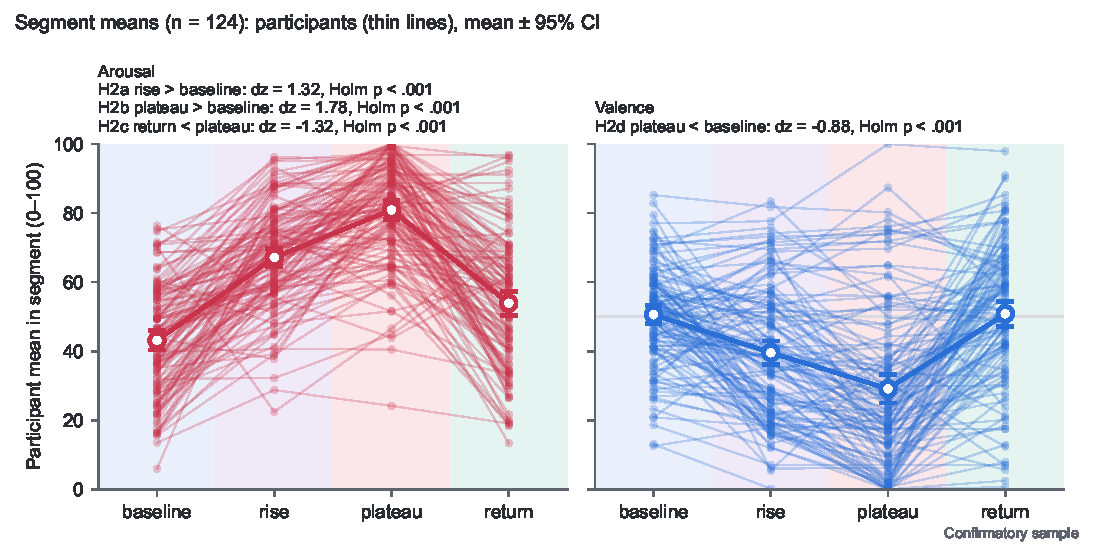
\includegraphics[width=\textwidth]{fig3_segment_means.pdf}
\caption{Mean ratings in the four preregistered segments (confirmatory sample, $N$~=~\val{n_primary}). Thin lines are
participants' segment means; the thick line shows group means with 95\% confidence intervals.}
\label{fig:segments}
\end{figure}

\begin{figure}[H]
\centering
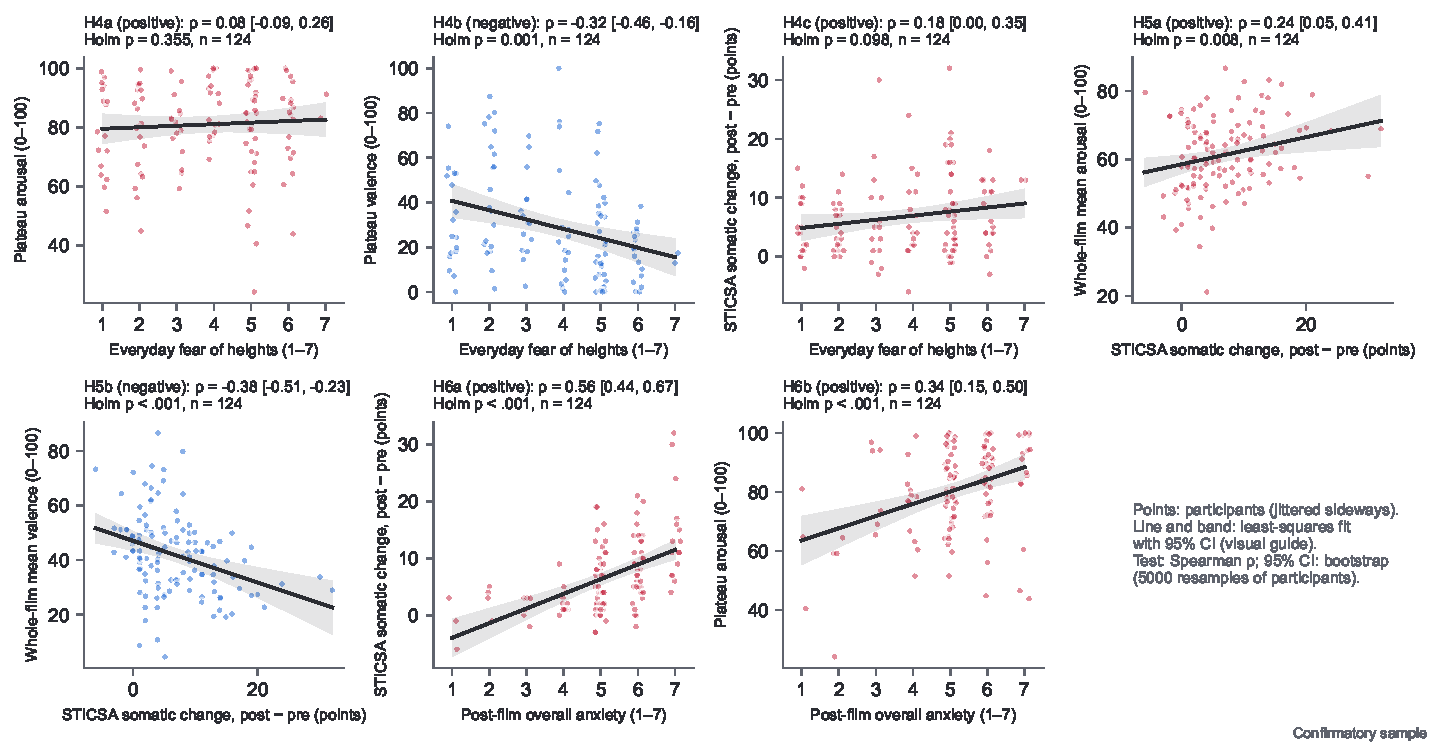
\includegraphics[width=\textwidth]{fig5_correlations.pdf}
\caption{Individual differences tested in H4--H6. Points are participants (jittered sideways); the black line and grey
band are a least-squares fit with its 95\% confidence interval, shown as a visual guide. Panel headings give Spearman
$\rho$ with bootstrap 95\% confidence intervals and Holm-adjusted $p$ values.}
\label{fig:correlations}
\end{figure}

\section*{S3. Registered Descriptive Analyses}

Split-half reliability of the group-mean series (1,000 random splits, Spearman--Brown corrected) was \val{rel:arousal}
for arousal and \val{rel:valence} for valence. Re-estimating the segment edges in the confirmatory sample with the
registered piecewise-linear method (three breakpoints, minimum segment length 30~s; 1,000 participant bootstrap
resamples) gave \val{edge1:est}~s \val{edge1:ci}, \val{edge2:est}~s \val{edge2:ci} and \val{edge3:est}~s
\val{edge3:ci}, against the registered \val{edge1:reg}, \val{edge2:reg} and \val{edge3:reg}~s. All tests used the fixed
registered edges.

\section*{S4. Exploratory Analyses}

The registration anticipated exploratory affect-grid and age/sex analyses without specifying confirmatory tests.
Figure~\ref{fig:grid} shows where on the affect grid participants spent their time in each segment. For age and sex
(Prolific profile data; $n$~=~\val{n_demo}
with both available), the STICSA change was regressed on sex and age, and segment means were modelled with a
random-intercept mixed model including segment (sum-coded) $\times$ (sex + age), with likelihood-ratio tests of the
interactions; the same model fitted by least squares with participant-clustered standard errors is reported as a check
(Table~\ref{tab:agesex}, Figures~\ref{fig:sexcourse} and \ref{fig:agesex}). The age/sex models were specified before
running them on the confirmatory sample; their $p$ values are uncorrected.

\begin{table}[tbp]
\caption{Exploratory Analyses of Age and Sex}
\label{tab:agesex}
\begin{threeparttable}
\footnotesize\linespread{1}\selectfont\setlength{\tabcolsep}{3.5pt}
\begin{tabular}{@{}llllll@{}}
\toprule
 & & \multicolumn{2}{l}{Main analysis} & \multicolumn{2}{l}{Clustered regression (check)} \\
\cmidrule(lr){3-4}\cmidrule(l){5-6}
Outcome & Effect & Test or estimate & $p$ & Test or estimate & $p$ \\
\midrule
STICSA change & Female $-$ male (points) & 0.66 [$-$1.77, 3.08] & .593 & -- & -- \\
 & Per 10 years of age (points) & 0.24 [$-$0.78, 1.25] & .645 & -- & -- \\
\addlinespace
Arousal & Segment $\times$ sex & $\chi^2$(3) = 0.28 & .964 & $F$(3, 120) = 0.08 & .969 \\
 & Segment $\times$ age & $\chi^2$(3) = 4.92 & .178 & $F$(3, 120) = 2.13 & .100 \\
 & Female $-$ male (film mean) & -- & -- & $-$0.50 [$-$4.47, 3.47] & .806 \\
 & Per 10 years (film mean) & -- & -- & $-$1.26 [$-$2.88, 0.37] & .129 \\
\addlinespace
Valence & Segment $\times$ sex & $\chi^2$(3) = 0.72 & .869 & $F$(3, 120) = 0.43 & .734 \\
 & Segment $\times$ age & $\chi^2$(3) = 1.84 & .607 & $F$(3, 120) = 0.50 & .682 \\
 & Female $-$ male (film mean) & -- & -- & $-$4.46 [$-$9.91, 0.99] & .108 \\
 & Per 10 years (film mean) & -- & -- & $-$0.74 [$-$2.96, 1.47] & .511 \\
\bottomrule
\end{tabular}
\vspace{4pt}
\begin{tablenotes}[para,flushleft]
{\small\textit{Note.} Exploratory analyses, not preregistered tests; $p$ values are uncorrected. $n$ = 121 participants of the primary sample with age and sex available. STICSA change: linear regression on sex and age. Segment means: random-intercept mixed model with segment (sum-coded) $\times$ (sex + age), interactions tested with likelihood-ratio tests (main analysis); the same model fitted by least squares with standard errors clustered by participant, interactions tested with Wald $F$ tests, is shown as a check, together with the main effects of sex and age averaged over the film. Age effects are per 10 years; sex effects are female minus male, in scale points.}
\end{tablenotes}
\end{threeparttable}
\end{table}


The change in each STICSA somatic item was examined after the confirmatory results were known (requested in review of
the draft): for each item, the mean change, the share of participants whose answer increased and $d_z$, with Wilcoxon
signed-rank tests Holm-corrected across the 11 items (Table~\ref{tab:items}).

\begin{table}[tbp]
\caption{Change in Each STICSA Somatic Item (Exploratory)}
\label{tab:items}
\begin{threeparttable}
\small\linespread{1}\selectfont
\begin{tabular}{@{}rlcccll@{}}
\toprule
Rank & Item & $M$ before & $M$ after & \% increased & $d_z$ [95\% CI] & $p_\mathrm{Holm}$ \\
\midrule
1 & Heart beats fast (item 1) & 1.43 & 2.57 & 73 & 1.17 [0.94, 1.40] & $<$ .001 \\
2 & Trembly, shaky (item 8) & 1.13 & 1.82 & 48 & 0.80 [0.60, 1.00] & $<$ .001 \\
3 & Breathing fast, shallow (item 18) & 1.17 & 1.81 & 50 & 0.77 [0.57, 0.97] & $<$ .001 \\
4 & Muscles tense (item 2) & 1.52 & 2.26 & 55 & 0.72 [0.52, 0.91] & $<$ .001 \\
5 & Dizzy (item 6) & 1.19 & 1.84 & 48 & 0.71 [0.51, 0.91] & $<$ .001 \\
6 & Face hot (item 12) & 1.15 & 1.69 & 40 & 0.66 [0.47, 0.86] & $<$ .001 \\
7 & Butterflies in stomach (item 20) & 1.18 & 1.74 & 42 & 0.64 [0.44, 0.83] & $<$ .001 \\
8 & Palms clammy (item 21) & 1.20 & 1.73 & 37 & 0.60 [0.40, 0.79] & $<$ .001 \\
9 & Throat dry (item 15) & 1.32 & 1.73 & 35 & 0.54 [0.35, 0.73] & $<$ .001 \\
10 & Muscles weak (item 7) & 1.22 & 1.62 & 35 & 0.52 [0.33, 0.71] & $<$ .001 \\
11 & Arms and legs stiff (item 14) & 1.26 & 1.74 & 37 & 0.52 [0.33, 0.71] & $<$ .001 \\
\bottomrule
\end{tabular}
\vspace{4pt}
\begin{tablenotes}[para,flushleft]
{\small\textit{Note.} Exploratory analysis, not a preregistered test. $N$ = 124 (primary confirmatory sample). Items answered from 1 (not at all) to 4 (very much so); short labels, original STICSA item numbers in parentheses. Ranked by $d_z$ (mean change divided by the standard deviation of the changes; exact 95\% CI). \% increased: share of participants whose answer was higher after the film. $p$ from Wilcoxon signed-rank tests, Holm-corrected across the 11 items.}
\end{tablenotes}
\end{threeparttable}
\end{table}


\begin{figure}[H]
\centering
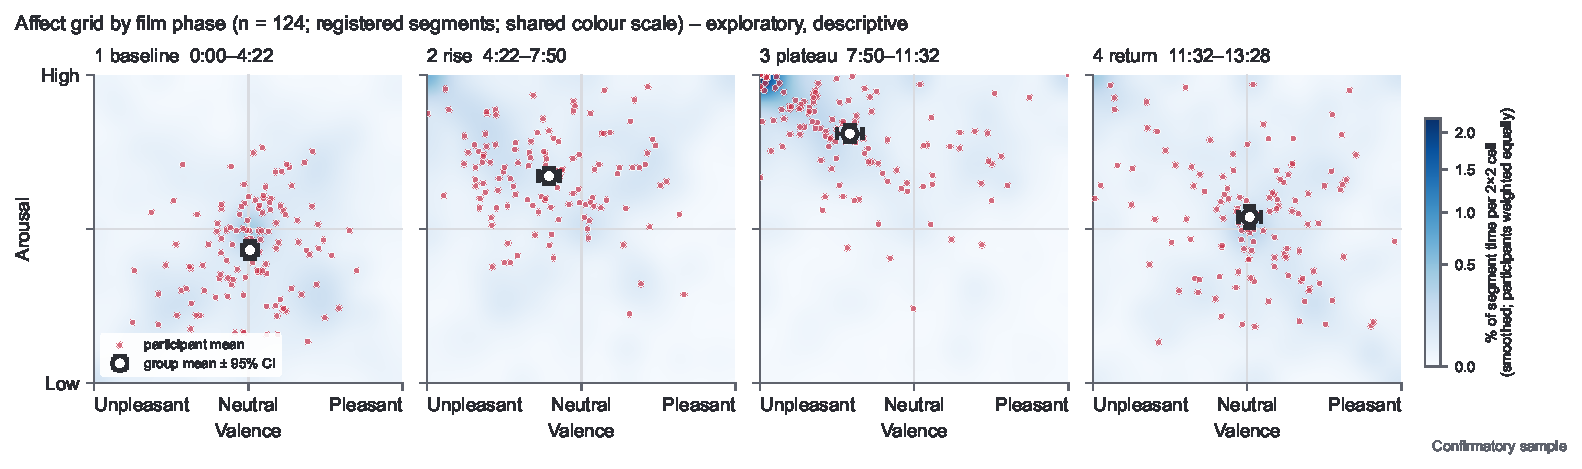
\includegraphics[width=\textwidth]{fig6_affect_grid_by_phase.pdf}
\caption{Occupancy of the affect grid in each segment (exploratory). Blue shading shows the share of viewing time in
each region (smoothed; participants weighted equally; same scale in all panels); dots are participants' mean ratings;
the open circle is the group mean with 95\% confidence intervals.}
\label{fig:grid}
\end{figure}

\begin{figure}[H]
\centering
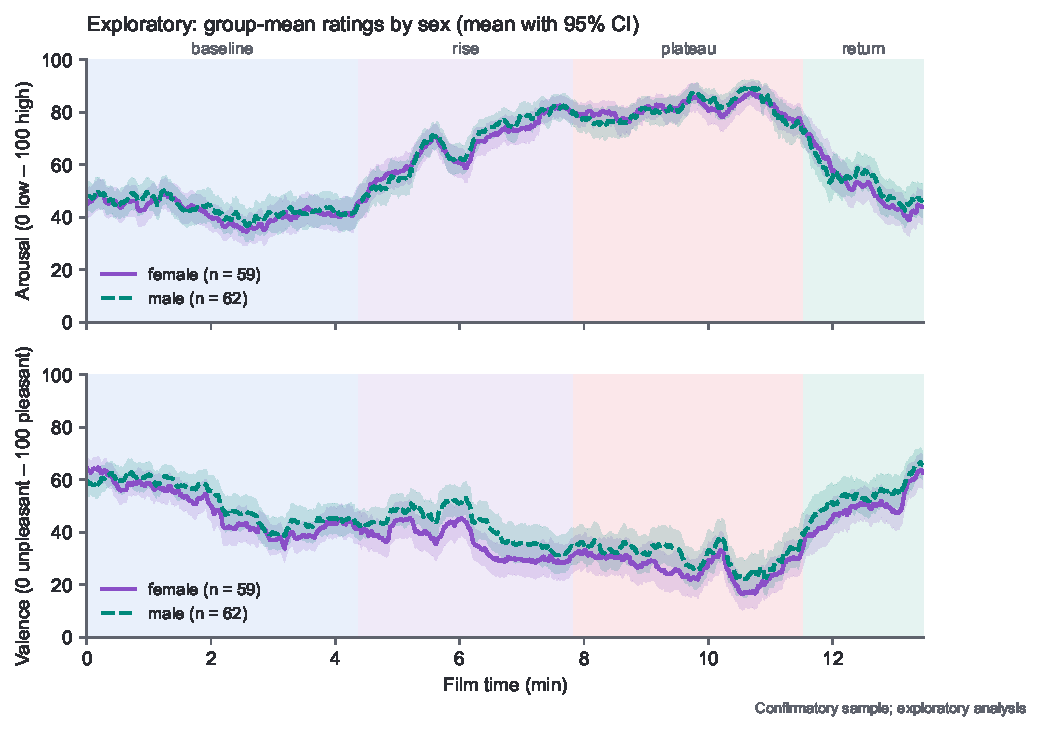
\includegraphics[width=\textwidth]{fig7_time_course_by_sex.pdf}
\caption{Group-mean ratings by sex (exploratory), with 95\% confidence intervals; female $n$~=~\val{n_demo_female}
(solid), male $n$~=~\val{n_demo_male} (dashed).}
\label{fig:sexcourse}
\end{figure}

\begin{figure}[H]
\centering
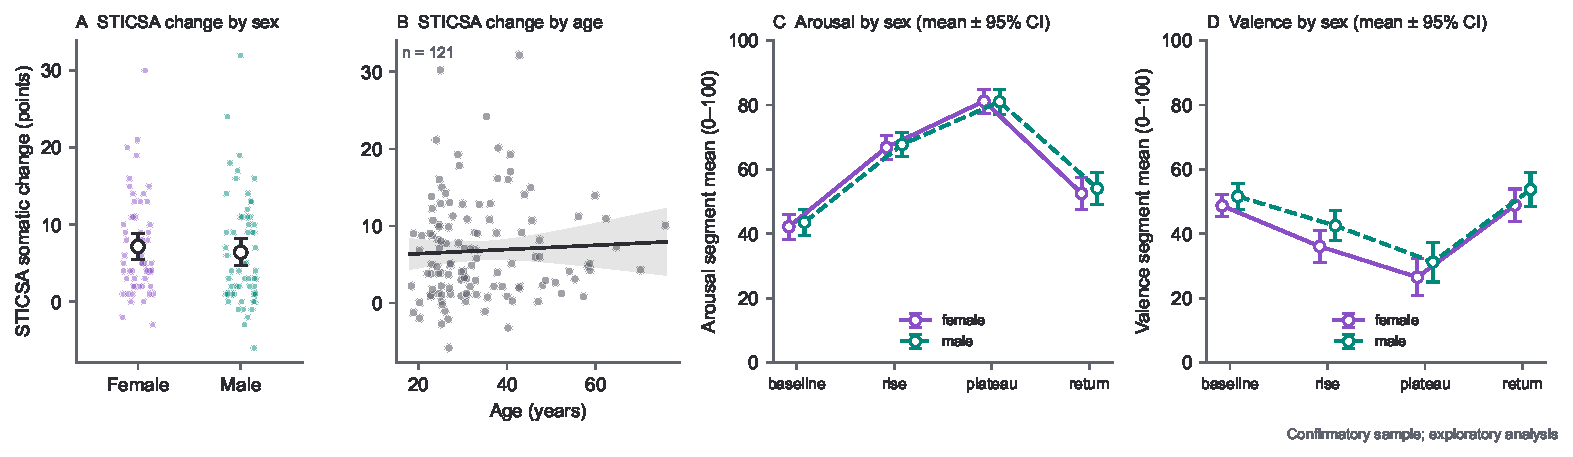
\includegraphics[width=\textwidth]{fig8_age_sex.pdf}
\caption{STICSA change by sex (A) and age (B; least-squares line with 95\% band as a visual guide), and segment means
by sex (C, D), exploratory; $n$~=~\val{n_demo}.}
\label{fig:agesex}
\end{figure}

\section*{S5. Notes on the Preregistered Plan}

H6 was added when preparing the registration, after inspection of a descriptive group-mean plot and before any
confirmatory hypothesis test. H1--H5 and their analysis plan were unchanged.

\begin{enumerate}
\item The registration reported 123 usable confirmatory participants at submission; one further participant completed
the study after that count, had complete data and passed all exclusion rules, and was included as registered
($N$~=~\val{n_primary}).
\item The fixed segment edges were estimated on 22 exploratory participants under the quality-control rules in use at
the time; under the final registered rules 21 are usable, and these form the reference curve for H3.
\item One participant's Prolific rejection was reversed for payment reasons; the participant
remains in the registered rejection set for the sensitivity analysis.
\item \enquote{Reported not watching attentively} was implemented as answering \enquote{No}; participants who answered
\enquote{Mostly} were retained.
\item Before the confirmatory run, the segment-edge bootstrap was set to 1,000 participant resamples; the
registration did not specify a number. Bootstraps used seed 20261004, and Spearman confidence intervals were
percentile intervals. H1 was treated as a single-test family, with the Wilcoxon check reported alongside; H3 was
decided by its confidence-interval criterion without a $p$ value.
\item Exploratory age and sex analyses used segment-level mixed models; models over the 1-Hz series, mentioned in
the registration as an example, were not implemented. Alternative optimisation algorithms were tried when needed
for convergence, without changing the model or decision rule.
\end{enumerate}

\end{document}
